% ============================================================================
% APPENDIX XV: LIT-HISTORY - Scientific History of Complementarity
% ============================================================================
% Category: LIT (Literature/Historical Analysis)
% Version: 1.0
% Status: Complete
% Prerequisites: VII (GTC), X (FORMAL-FOUND), XIV (DOMAIN-CATALOG)
% ============================================================================

\begin{chapter}{Scientific History of Complementarity: From Ontological Tension to Formal Interaction}
\label{app:lit-history}

% ============================================================================
% HEADER BLOCK
% ============================================================================
\begin{tcolorbox}[colback=gray!5!white,colframe=gray!75!black]
\small
\textbf{Category:} LIT (Literature/Historical Analysis) \\
\textbf{Code:} XV \\
\textbf{Version:} 1.0 \\
\textbf{Status:} Complete \\
\textbf{Dependencies:} VII (GTC), X (FORMAL-FOUND), XIV (DOMAIN-CATALOG) \\
\textbf{Provides Foundation For:} All FORMAL and DOMAIN appendices
\end{tcolorbox}

% ============================================================================
% CROSS-REFERENCE MAP
% ============================================================================
\begin{tcolorbox}[colback=blue!5!white,colframe=blue!75!black,title=\textbf{Cross-Reference Map}]
\small
\textbf{This appendix relates to:}
\begin{itemize}[noitemsep]
    \item \textbf{VII (GTC):} The formal theory this history leads to
    \item \textbf{X (FORMAL-FOUND):} Mathematical foundations emerging from this history
    \item \textbf{XI (FORMAL-MODELS):} Canonical models as historical culmination
    \item \textbf{XIV (DOMAIN-CATALOG):} Cross-disciplinary applications
    \item \textbf{K (LIT-FEHR):} Fehr's contribution to behavioral complementarity
    \item \textbf{L (LIT-KAHNEMAN):} Kahneman's dual-system interactions
\end{itemize}
\end{tcolorbox}

% ============================================================================
% ABSTRACT
% ============================================================================
\begin{abstract}
This appendix provides a rigorous scientific history of complementarity---tracing its evolution from pre-scientific ontological intuitions through classical marginalization, quantum-mechanical epistemology, systems-theoretic implicitness, disciplinary fragmentation, to contemporary formal unification. We identify five critical phases: (I) ontological foundations, (II) reductionist suppression, (III) Bohrian epistemological articulation, (IV) systems-theoretic latency, and (V) formal island emergence. The analysis reveals why complementarity remained scientifically underdeveloped despite intuitive plausibility, and why the current moment---characterized by computational power, network theory, and cross-disciplinary data---enables the first unified theory of complementarity ($\gamma$). This historical reconstruction positions the EBF framework as the culmination of a 2,500-year intellectual trajectory.
\end{abstract}

% ============================================================================
% QUICK REFERENCE
% ============================================================================
\begin{tcolorbox}[colback=yellow!5!white,colframe=yellow!75!black,title=\textbf{Quick Reference: Historical Phases}]
\small
\renewcommand{\arraystretch}{1.2}
\begin{tabular}{@{}clll@{}}
\toprule
\textbf{Phase} & \textbf{Period} & \textbf{Status} & \textbf{Key Figure} \\
\midrule
I & Antiquity--17th c. & Metaphysical & Heraclitus, Aristotle \\
II & 17th--19th c. & Marginalized & Newton, Laplace \\
III & 1920s--1930s & Epistemological & Bohr \\
IV & 1940s--1970s & Implicit & Wiener, Bertalanffy \\
V & 1970s--1990s & Fragmented & Topkis, Milgrom \\
VI & 2000--present & Unifying & EBF $\gamma$-framework \\
\bottomrule
\end{tabular}
\end{tcolorbox}

% ============================================================================
% FUNDAMENTAL QUESTION
% ============================================================================
\begin{tcolorbox}[colback=red!5!white,colframe=red!75!black,title=\textbf{Fundamental Question}]
\textbf{Why did it take 2,500 years from the first intuitions about complementarity to the development of a formal, unified, cross-disciplinary theory?}

This appendix answers this question through rigorous historical analysis.
\end{tcolorbox}

% ============================================================================
% PART I: PRE-SCIENTIFIC PHASE
% ============================================================================
\section{Phase I: Pre-Scientific Foundations}
\label{sec:phase-i}

\subsection{Complementarity as Ontological Grundmotiv (Antiquity--17th Century)}

\begin{tcolorbox}[colback=purple!5!white,colframe=purple!75!black,title=\textbf{Core Thesis}]
The world is not constructed from isolated units, but from mutually completing opposites. This intuition appeared across cultures but remained:
\begin{itemize}[noitemsep]
    \item Qualitative (not quantitative)
    \item Non-measurable
    \item Non-operationalizable
\end{itemize}
\textbf{Epistemic Status:} $\square$ Metaphysical, not scientific
\end{tcolorbox}

\subsubsection{Greek Foundations}

\textbf{Heraclitus (c. 535--475 BCE)}

The \textit{unity of opposites} (\textgreek{ἑνότης τῶν ἐναντίων}) represents the earliest articulation of complementarity:

\begin{quote}
``The road up and the road down is one and the same.'' (Fragment 60)
\end{quote}

\begin{quote}
``Opposition brings concord. Out of discord comes the fairest harmony.'' (Fragment 8)
\end{quote}

\textbf{Key insight:} Opposites are not merely co-present but \textit{constitutively interdependent}. The value of one depends on the other.

\textbf{Limitation:} No mechanism, no measurement, no prediction.

\vspace{0.5em}
\textbf{Aristotle (384--322 BCE)}

Aristotelian metaphysics provides multiple complementarity structures:

\begin{table}[h]
\centering
\caption{Aristotelian Complementary Pairs}
\label{tab:aristotle-pairs}
\renewcommand{\arraystretch}{1.2}
\begin{tabular}{@{}lll@{}}
\toprule
\textbf{Pair} & \textbf{Greek} & \textbf{Complementarity Type} \\
\midrule
Form--Matter & \textgreek{μορφή}--\textgreek{ὕλη} & Constitutive \\
Potency--Act & \textgreek{δύναμις}--\textgreek{ἐνέργεια} & Dynamic \\
Final--Efficient Cause & \textgreek{τέλος}--\textgreek{κίνησις} & Explanatory \\
\bottomrule
\end{tabular}
\end{table}

\textbf{Critical observation:} Aristotle recognizes that form without matter is empty, matter without form is indeterminate. Neither is sufficient alone.

This is \textit{proto-complementarity}: $\gamma_{\text{form,matter}} > 0$ in modern notation.

\subsubsection{Eastern Traditions}

\textbf{Yin-Yang (China, c. 700 BCE onwards)}

The most systematic pre-scientific complementarity framework:

\begin{itemize}[noitemsep]
    \item Two principles, neither complete alone
    \item Dynamic balance, not static opposition
    \item Mutual transformation (Yin contains Yang-seed)
    \item Application across medicine, governance, cosmology
\end{itemize}

\textbf{Modern interpretation:}
\[
\gamma_{\text{Yin,Yang}} = U(\text{Yin} \cup \text{Yang}) - U(\text{Yin}) - U(\text{Yang}) > 0
\]

The whole exceeds the sum of parts---the defining characteristic of positive complementarity.

\subsubsection{Medieval Scholasticism}

Scholastic philosophy preserved and formalized Greek complementarity concepts:

\begin{itemize}[noitemsep]
    \item \textbf{Thomas Aquinas:} Soul-body unity (neither sufficient alone)
    \item \textbf{Duns Scotus:} Formal distinction without real separation
    \item \textbf{Nicholas of Cusa:} \textit{Coincidentia oppositorum} (coincidence of opposites)
\end{itemize}

\begin{quote}
``In God, all opposites coincide.'' ---Nicholas of Cusa, \textit{De docta ignorantia} (1440)
\end{quote}

\subsubsection{Phase I Assessment}

\begin{table}[h]
\centering
\caption{Phase I: Pre-Scientific Complementarity}
\label{tab:phase-i-assessment}
\renewcommand{\arraystretch}{1.3}
\begin{tabular}{@{}lcc@{}}
\toprule
\textbf{Criterion} & \textbf{Status} & \textbf{Modern Equivalent} \\
\midrule
Intuitive recognition & \checkmark & Acknowledged \\
Cross-cultural presence & \checkmark & Acknowledged \\
Qualitative description & \checkmark & Necessary but insufficient \\
Formal definition & $\times$ & $\gamma_{ab} = f(\{a,b\}) - f(\{a\}) - f(\{b\}) + f(\emptyset)$ \\
Measurement procedure & $\times$ & Factorial designs, SHAP \\
Testable predictions & $\times$ & Comparative statics theorems \\
Operational guidance & $\times$ & Intervention complementarity \\
\bottomrule
\end{tabular}
\end{table}

\textbf{Verdict:} Phase I established complementarity as an \textit{ontological intuition} but provided no scientific infrastructure.

% ============================================================================
% PART II: CLASSICAL SCIENCE
% ============================================================================
\section{Phase II: Classical Science and Reductionist Suppression}
\label{sec:phase-ii}

\subsection{The Newtonian Revolution (17th--19th Century)}

\begin{tcolorbox}[colback=orange!5!white,colframe=orange!75!black,title=\textbf{Critical Historical Event}]
The Newtonian revolution established \textbf{additive decomposition} as the gold standard of scientific explanation. This paradigm systematically marginalized complementarity.
\end{tcolorbox}

\subsubsection{The Reductionist Paradigm}

\textbf{Core assumptions of classical science:}

\begin{enumerate}
    \item \textbf{Decomposability:} Complex systems = sum of simple parts
    \[
    \text{System} = \sum_{i} \text{Component}_i
    \]

    \item \textbf{Linear causality:} Effects proportional to causes
    \[
    \text{Effect} = k \cdot \text{Cause}
    \]

    \item \textbf{Interaction as perturbation:} Interactions are disturbances, not structure
    \[
    f(x,y) \approx f_x(x) + f_y(y) + \epsilon
    \]
    where $\epsilon$ is ``noise'' to be minimized
\end{enumerate}

\textbf{Laplacian determinism (1814):}
\begin{quote}
``An intellect which at a certain moment would know all forces [...] would embrace in a single formula the movements of the greatest bodies of the universe and those of the tiniest atom.''
\end{quote}

\textbf{Implication:} If everything reduces to particles and forces, there is no room for emergent complementarity.

\subsubsection{Why Complementarity Was Marginalized}

\begin{table}[h]
\centering
\caption{Reductionism vs. Complementarity}
\label{tab:reductionism-complementarity}
\renewcommand{\arraystretch}{1.3}
\begin{tabular}{@{}lcc@{}}
\toprule
\textbf{Feature} & \textbf{Reductionism} & \textbf{Complementarity} \\
\midrule
Ontology & Parts fundamental & Relations fundamental \\
Explanation & Bottom-up only & Top-down possible \\
Mathematics & Linear algebra & Nonlinear, set functions \\
Interactions & Residual & Structural \\
Complexity & Reducible & Emergent \\
\bottomrule
\end{tabular}
\end{table}

\textbf{Institutional consequences:}
\begin{itemize}[noitemsep]
    \item Complementarity viewed as ``fuzzy,'' ``unscientific''
    \item Holistic approaches relegated to philosophy
    \item No mathematical tools for interaction analysis
    \item Training emphasized decomposition, not synthesis
\end{itemize}

\subsubsection{Exception Islands}

Despite reductionist dominance, complementarity survived in specialized domains:

\textbf{1. Chemistry: Stoichiometry}
\begin{itemize}[noitemsep]
    \item Compounds $\neq$ mixtures
    \item $2H_2 + O_2 \to 2H_2O$ (emergent properties)
    \item But: No general theory of chemical complementarity
\end{itemize}

\textbf{2. Biology: Organism Concept}
\begin{itemize}[noitemsep]
    \item Organs interdependent (heart needs lungs, lungs need blood)
    \item Cuvier's ``correlation of parts'' (1812)
    \item But: Descriptive, not mathematical
\end{itemize}

\textbf{3. Economics: Early Intuitions}
\begin{itemize}[noitemsep]
    \item Complementary goods (carriages and horses)
    \item Cournot (1838): First mathematical treatment
    \item But: Isolated results, no unified framework
\end{itemize}

\subsubsection{Phase II Assessment}

\begin{tcolorbox}[colback=red!5!white,colframe=red!75!black,title=\textbf{Phase II Verdict}]
\textbf{Epistemic Status:} Complementarity \textit{epistemically marginalized}

The reductionist paradigm achieved enormous success in physics, creating a path dependency that:
\begin{enumerate}[noitemsep]
    \item Defined ``scientific'' as ``decomposable''
    \item Made interactions seem like failures of analysis
    \item Provided no mathematical language for complementarity
    \item Created institutional barriers to holistic approaches
\end{enumerate}

\textbf{Result:} Two centuries of scientific progress with systematic neglect of complementarity.
\end{tcolorbox}

% ============================================================================
% PART III: BOHRIAN TURN
% ============================================================================
\section{Phase III: The Bohrian Epistemological Turn}
\label{sec:phase-iii}

\subsection{Quantum Complementarity (1920s--1930s)}

\begin{tcolorbox}[colback=green!5!white,colframe=green!75!black,title=\textbf{Historical Turning Point}]
Niels Bohr's complementarity principle (1927) represents the first \textit{scientific} articulation of complementarity---but as an \textbf{epistemological}, not ontological, concept.
\end{tcolorbox}

\subsubsection{Bohr's Complementarity Principle}

\textbf{The Problem:} Quantum entities exhibit both wave-like and particle-like behavior, but these cannot be observed simultaneously.

\textbf{Bohr's Solution (Como Lecture, 1927):}

\begin{quote}
``The very nature of the quantum theory [...] forces us to regard the space-time coordination and the claim of causality, the union of which characterizes the classical theories, as complementary but exclusive features of the description.''
\end{quote}

\textbf{Key features:}
\begin{enumerate}
    \item \textbf{Mutual exclusivity:} Wave and particle descriptions cannot be applied simultaneously
    \item \textbf{Joint necessity:} Both are required for complete description
    \item \textbf{Observation dependence:} The experimental setup determines which aspect manifests
\end{enumerate}

\subsubsection{Critical Distinction from Modern $\gamma$}

\begin{table}[h]
\centering
\caption{Bohrian vs. EBF Complementarity}
\label{tab:bohr-vs-ebf}
\renewcommand{\arraystretch}{1.3}
\begin{tabular}{@{}lcc@{}}
\toprule
\textbf{Feature} & \textbf{Bohr} & \textbf{EBF $\gamma$} \\
\midrule
Type & Epistemological & Ontological \\
Focus & Description limits & Value creation \\
Domain & Quantum physics & All domains \\
Measurable & No & Yes \\
Interaction & Not applicable & Core concept \\
Formula & None & $\gamma_{ab} = f(\{a,b\}) - f(\{a\}) - f(\{b\}) + f(\emptyset)$ \\
\bottomrule
\end{tabular}
\end{table}

\textbf{Bohr's own clarification:}
\begin{quote}
``Complementarity is a feature of our \textit{description}, not of nature itself.''
\end{quote}

This is crucial: Bohr's complementarity concerns the \textit{limits of simultaneous knowledge}, not the \textit{interaction of combined elements}.

\subsubsection{Philosophical Reception}

Bohr's principle triggered extensive philosophical discussion:

\begin{itemize}[noitemsep]
    \item \textbf{Copenhagen interpretation:} Complementarity as fundamental epistemological limit
    \item \textbf{Heisenberg:} Connection to uncertainty relations
    \item \textbf{Pauli:} Extension to psychology (synchronicity with Jung)
    \item \textbf{Critics (Einstein, Schrödinger):} Incompleteness objections
\end{itemize}

\textbf{Paradox:} Despite enormous philosophical impact, Bohr's complementarity generated almost no \textit{methodological} generalization.

\subsubsection{Why Bohrian Complementarity Didn't Generalize}

\begin{enumerate}
    \item \textbf{Too specific:} Tied to quantum measurement problem
    \item \textbf{Non-quantitative:} No formula, no measurement procedure
    \item \textbf{Negative definition:} About what \textit{cannot} be done simultaneously
    \item \textbf{No interaction concept:} Wave and particle don't ``interact''
    \item \textbf{Philosophical ownership:} Became property of philosophy of physics
\end{enumerate}

\subsubsection{Phase III Assessment}

\begin{tcolorbox}[colback=yellow!5!white,colframe=yellow!75!black,title=\textbf{Phase III Verdict}]
\textbf{Epistemic Status:} $\square$ Epistemological, not ontological; $\square$ Not operationalized

Bohr legitimized ``complementarity'' as a scientific term but defined it in ways that:
\begin{itemize}[noitemsep]
    \item Made it seem quantum-specific
    \item Emphasized limits rather than possibilities
    \item Provided no framework for other domains
    \item Created terminological confusion (complementarity $\neq$ interaction)
\end{itemize}

\textbf{Lasting impact:} The word ``complementarity'' entered scientific vocabulary, but its Bohrian meaning actually \textit{impeded} generalization.
\end{tcolorbox}

% ============================================================================
% PART IV: SYSTEMS THEORY
% ============================================================================
\section{Phase IV: Systems Theory and Implicit Complementarity}
\label{sec:phase-iv}

\subsection{Cybernetics and General Systems Theory (1940s--1970s)}

\begin{tcolorbox}[colback=blue!5!white,colframe=blue!75!black,title=\textbf{Structural Presence, Conceptual Absence}]
Systems theory recognized that system behavior emerges from component interactions. Yet complementarity remained \textbf{implicit}---structurally present but not named, measured, or theorized.
\end{tcolorbox}

\subsubsection{Key Figures and Concepts}

\textbf{Norbert Wiener (1894--1964): Cybernetics}
\begin{itemize}[noitemsep]
    \item Feedback loops create emergent stability
    \item System $\neq$ sum of parts
    \item But: Focus on control, not complementarity per se
\end{itemize}

\textbf{Ludwig von Bertalanffy (1901--1972): General Systems Theory}
\begin{itemize}[noitemsep]
    \item ``The whole is more than the sum of its parts''
    \item Isomorphic structures across domains
    \item But: No formal definition of ``more than''
\end{itemize}

\textbf{W. Ross Ashby (1903--1972): Requisite Variety}
\begin{itemize}[noitemsep]
    \item System complexity requires matching control complexity
    \item Implicit complementarity between system and controller
    \item But: No $\gamma$ metric
\end{itemize}

\subsubsection{Why Complementarity Remained Implicit}

\begin{table}[h]
\centering
\caption{Systems Theory: Implicit Complementarity}
\label{tab:systems-implicit}
\renewcommand{\arraystretch}{1.3}
\begin{tabular}{@{}lcc@{}}
\toprule
\textbf{Concept} & \textbf{Complementarity Present?} & \textbf{Explicitly Named?} \\
\midrule
Feedback loops & Yes (circular causation) & No \\
Emergence & Yes ($\gamma > 0$) & No (vague ``more than'') \\
Homeostasis & Yes (component interdependence) & No \\
Hierarchy & Yes (level interactions) & No \\
Autopoiesis & Yes (self-creating complementarity) & No \\
\bottomrule
\end{tabular}
\end{table}

\textbf{Reasons for non-articulation:}
\begin{enumerate}
    \item \textbf{Focus on stability:} Interest in equilibrium, not interaction values
    \item \textbf{Qualitative emphasis:} Mathematical formalization resisted
    \item \textbf{Anti-reductionist stance:} Opposition defined identity, not positive theory
    \item \textbf{No measurement tradition:} Emerged from biology, not economics
\end{enumerate}

\subsubsection{Luhmann and Social Systems}

Niklas Luhmann's social systems theory (1984) represents the most sophisticated implicit complementarity:

\begin{itemize}[noitemsep]
    \item Systems constitute themselves through difference
    \item System/environment complementarity fundamental
    \item Structural coupling between systems
\end{itemize}

\textbf{Modern translation:}
\[
\gamma_{\text{system,environment}} = \text{Operational closure} + \text{Structural coupling}
\]

But Luhmann never quantified these relationships.

\subsubsection{Phase IV Assessment}

\begin{tcolorbox}[colback=orange!5!white,colframe=orange!75!black,title=\textbf{Phase IV Verdict}]
\textbf{Epistemic Status:} $\square$ Structurally present; $\square$ Conceptually unclear

Systems theory:
\begin{itemize}[noitemsep]
    \item Correctly identified that interactions create emergent properties
    \item Failed to provide operational definitions
    \item Generated resistance from quantitative sciences
    \item Left complementarity as an intuition, not a tool
\end{itemize}

\textbf{Legacy:} Rehabilitated holistic thinking but without the formal apparatus to make it scientific.
\end{tcolorbox}

% ============================================================================
% PART V: FORMAL ISLANDS
% ============================================================================
\section{Phase V: Emergence of Formal Islands}
\label{sec:phase-v}

\subsection{Disciplinary Formalization (1970s--1990s)}

\begin{tcolorbox}[colback=green!5!white,colframe=green!75!black,title=\textbf{The Fragmentation Paradox}]
The late 20th century saw rigorous formalization of complementarity---but in isolated disciplinary islands with no cross-domain communication.
\end{tcolorbox}

\subsubsection{Island 1: Economics}

\textbf{Wassily Leontief (1906--1999): Input-Output Analysis}
\begin{itemize}[noitemsep]
    \item Complementary inputs in production
    \item Fixed coefficients (Leontief production function)
    \item Nobel Prize 1973
\end{itemize}

\textbf{Donald Topkis (1940--2013): Supermodularity}
\begin{itemize}[noitemsep]
    \item Formal definition of complementarity on lattices (1978)
    \item Monotone comparative statics
    \item Definitive monograph (1998)
\end{itemize}

\begin{definition}[Topkis Supermodularity]
A function $f: 2^S \to \mathbb{R}$ is supermodular if:
\[
f(A \cup B) + f(A \cap B) \geq f(A) + f(B) \quad \forall A, B \subseteq S
\]
\end{definition}

\textbf{Paul Milgrom \& John Roberts: Strategic Complementarity}
\begin{itemize}[noitemsep]
    \item ``The Economics of Modern Manufacturing'' (1990)
    \item ``Complementarities and fit'' (1995)
    \item Applied to organizational design
\end{itemize}

\begin{quote}
``Resistance to [strategic] changes arises because a resistance to change in any practice reduces the value of the other changes.'' ---Milgrom \& Roberts (1990)
\end{quote}

\textbf{Epistemic Status:} $\checkmark$ Formal; $\checkmark$ Measurable; $\times$ Domain-specific

\subsubsection{Island 2: Biology}

\textbf{Epistasis}
\begin{itemize}[noitemsep]
    \item Non-additive gene interactions
    \item $\gamma_{AB} = \text{Fitness}(AB) - \text{Fitness}(A) - \text{Fitness}(B) + \text{Fitness}(\emptyset)$
    \item Extensive empirical documentation
    \item Fisher (1918), Phillips (2008)
\end{itemize}

\textbf{Cooperativity}
\begin{itemize}[noitemsep]
    \item Binding site interactions (Hill equation, 1910)
    \item Allosteric regulation (Monod, Wyman, Changeux, 1965)
    \item Quantified via Hill coefficient
\end{itemize}

\textbf{Ecological Synergies}
\begin{itemize}[noitemsep]
    \item Species complementarity in ecosystems
    \item Biodiversity-productivity relationships
    \item Tilman et al. (1996): Biodiversity and stability
\end{itemize}

\textbf{Epistemic Status:} $\checkmark$ Empirically rich; $\times$ No unified theory

\subsubsection{Island 3: Pharmacology}

\textbf{Drug Synergy}
\begin{itemize}[noitemsep]
    \item Combination therapy (HIV, cancer, antibiotics)
    \item Chou-Talalay method: Combination Index (1984)
    \item Bliss independence, Loewe additivity
\end{itemize}

\begin{definition}[Combination Index]
\[
CI = \frac{d_1}{D_{x,1}} + \frac{d_2}{D_{x,2}}
\]
where $CI < 1$ indicates synergy, $CI > 1$ antagonism.
\end{definition}

\textbf{Epistemic Status:} $\checkmark$ Practically essential; $\times$ Isolated methodology

\subsubsection{Island 4: Computer Science}

\textbf{Submodular Optimization}
\begin{itemize}[noitemsep]
    \item Greedy algorithms with guarantees (Nemhauser, Wolsey, Fisher, 1978)
    \item Machine learning applications (feature selection)
    \item Active research community (Krause, Vondrák, Karbasi)
\end{itemize}

\textbf{Epistemic Status:} $\checkmark$ Algorithmically sophisticated; $\times$ No domain theory

\subsubsection{The Fragmentation Problem}

\begin{table}[h]
\centering
\caption{Formal Islands: Same Structure, Different Vocabularies}
\label{tab:formal-islands}
\renewcommand{\arraystretch}{1.3}
\begin{tabular}{@{}llll@{}}
\toprule
\textbf{Domain} & \textbf{Term} & \textbf{Formula} & \textbf{Community} \\
\midrule
Economics & Complementarity & Supermodularity & Econometrica \\
Biology & Epistasis & Fitness landscape & Nature Genetics \\
Pharmacology & Synergy & Combination Index & Pharmacology \\
Computer Science & Submodularity & Set function & NeurIPS \\
Psychology & Interaction & ANOVA interaction & Psych Methods \\
\bottomrule
\end{tabular}
\end{table}

\textbf{The problem:} Each island developed sophisticated tools but:
\begin{itemize}[noitemsep]
    \item Used different terminology
    \item Published in different venues
    \item Had no awareness of isomorphism
    \item Never attempted unification
\end{itemize}

\subsubsection{Phase V Assessment}

\begin{tcolorbox}[colback=purple!5!white,colframe=purple!75!black,title=\textbf{Phase V Verdict}]
\textbf{Epistemic Status:} $\checkmark$ Formal in islands; $\times$ Globally fragmented

The late 20th century achieved what earlier phases could not:
\begin{itemize}[noitemsep]
    \item Rigorous mathematical definitions
    \item Quantitative measurement procedures
    \item Testable empirical predictions
\end{itemize}

But it failed to achieve:
\begin{itemize}[noitemsep]
    \item Cross-domain recognition
    \item Unified terminology
    \item General theory
\end{itemize}

\textbf{Historical irony:} The same mathematical structure ($\gamma = f(A \cup B) - f(A) - f(B) + f(\emptyset)$) was discovered independently 5+ times without anyone noticing.
\end{tcolorbox}

% ============================================================================
% PART VI: 21ST CENTURY PARADOX
% ============================================================================
\section{Phase VI: The 21st Century Paradox}
\label{sec:phase-vi}

\subsection{Complementarity Everywhere, Theory Nowhere}

\begin{tcolorbox}[colback=red!5!white,colframe=red!75!black,title=\textbf{The Contemporary Bottleneck}]
In the early 21st century, complementarity has become central to:
\begin{itemize}[noitemsep]
    \item Machine learning (feature interactions)
    \item Neuroscience (functional connectivity)
    \item Ecology (biodiversity-function relationships)
    \item Sociology (network effects)
    \item Management (organizational complementarities)
\end{itemize}

Yet: Each discipline continues to ``invent'' its own vocabulary with no shared metric and no theoretical ordering.
\end{tcolorbox}

\subsubsection{Evidence of Centrality}

\textbf{Machine Learning}
\begin{itemize}[noitemsep]
    \item SHAP values explicitly decompose interactions
    \item Neural network interpretability focuses on feature complementarity
    \item Causal discovery increasingly interaction-focused
\end{itemize}

\textbf{Neuroscience}
\begin{itemize}[noitemsep]
    \item Functional connectivity = $\gamma$ between brain regions
    \item Integration-segregation balance fundamental
    \item Connectomics entirely about interaction structure
\end{itemize}

\textbf{Ecology}
\begin{itemize}[noitemsep]
    \item Species complementarity drives ecosystem function
    \item Biodiversity experiments measure $\gamma_{\text{species}}$
    \item Trophic interactions create emergent stability
\end{itemize}

\subsubsection{The Vocabulary Babel}

\begin{table}[h]
\centering
\caption{One Concept, Many Names (2020s)}
\label{tab:vocabulary-babel}
\renewcommand{\arraystretch}{1.2}
\small
\begin{tabular}{@{}lll@{}}
\toprule
\textbf{Domain} & \textbf{Term for $\gamma > 0$} & \textbf{Term for $\gamma < 0$} \\
\midrule
Economics & Complementarity & Substitutability \\
Biology & Epistasis, Cooperativity & Antagonism \\
Pharmacology & Synergy & Antagonism \\
Psychology & Interaction effect & Interference \\
Neuroscience & Functional connectivity & Competition \\
Ecology & Facilitation & Inhibition \\
ML/Statistics & Interaction & Redundancy \\
Sociology & Network externality & Crowding-out \\
\bottomrule
\end{tabular}
\end{table}

\textbf{Consequence:} Researchers in different fields cannot recognize they are studying the same phenomenon.

\subsubsection{Why Unification Hasn't Happened}

\begin{enumerate}
    \item \textbf{Institutional barriers:}
    \begin{itemize}[noitemsep]
        \item Disciplinary silos reinforce separation
        \item Journals specialized by field
        \item Career incentives favor depth over breadth
    \end{itemize}

    \item \textbf{Mathematical barriers:}
    \begin{itemize}[noitemsep]
        \item Combinatorial explosion with higher-order $\gamma$
        \item Identification requires exponentially large datasets
        \item No standard estimation methodology
    \end{itemize}

    \item \textbf{Philosophical barriers:}
    \begin{itemize}[noitemsep]
        \item Reductionism still dominates training
        \item Interactions seen as ``residuals''
        \item No perceived need for unification
    \end{itemize}
\end{enumerate}

% ============================================================================
% PART VII: WHY NO GENERAL THEORY EXISTED
% ============================================================================
\section{Phase VII: Explaining the Historical Lacuna}
\label{sec:phase-vii}

\subsection{Why It Took 2,500 Years}

\begin{tcolorbox}[colback=gray!5!white,colframe=gray!75!black,title=\textbf{Three Types of Barriers}]
The absence of a unified complementarity theory resulted from the confluence of:
\begin{enumerate}
    \item \textbf{Methodological barriers} (how to measure)
    \item \textbf{Epistemic barriers} (how to think)
    \item \textbf{Institutional barriers} (how knowledge is organized)
\end{enumerate}
\end{tcolorbox}

\subsubsection{Methodological Barriers}

\textbf{Problem 1: Combinatorial Explosion}

For $n$ elements, full characterization requires:
\[
\text{Parameters} = 2^n - 1
\]

For $n = 20$ elements: over 1 million interaction parameters.

\textbf{Problem 2: Identification}

To estimate $\gamma_{ab}$, one needs:
\begin{itemize}[noitemsep]
    \item Observations of $\{a,b\}$ together
    \item Observations of $\{a\}$ alone
    \item Observations of $\{b\}$ alone
    \item Observations of $\{\emptyset\}$
\end{itemize}

This requires factorial designs that grow exponentially.

\textbf{Problem 3: Higher-Order Identification}

For $\gamma_{abc}$, one needs:
\[
\gamma_{abc} = f(\{a,b,c\}) - f(\{a,b\}) - f(\{a,c\}) - f(\{b,c\}) + f(\{a\}) + f(\{b\}) + f(\{c\}) - f(\emptyset)
\]

Eight terms, requiring eight distinct observations.

\subsubsection{Epistemic Barriers}

\textbf{The Reductionist Training Problem}

Scientific education systematically trains:
\begin{itemize}[noitemsep]
    \item Linear thinking (effects proportional to causes)
    \item Ceteris paribus reasoning (isolate variables)
    \item Main effect focus (interactions are ``complications'')
\end{itemize}

\textbf{Result:} Generations of scientists trained to see interactions as noise, not signal.

\textbf{The ``Residual'' Framing}

In standard statistical training:
\[
Y = \beta_0 + \beta_1 X_1 + \beta_2 X_2 + \underbrace{\beta_{12} X_1 X_2}_{\text{``optional''}} + \epsilon
\]

The interaction term is presented as:
\begin{itemize}[noitemsep]
    \item Added only if necessary
    \item A complication, not a feature
    \item Secondary to ``main effects''
\end{itemize}

\subsubsection{Institutional Barriers}

\textbf{Disciplinary Silos}
\begin{itemize}[noitemsep]
    \item Economists don't read neuroscience journals
    \item Biologists don't attend operations research conferences
    \item No venue for ``complementarity science''
\end{itemize}

\textbf{Career Incentives}
\begin{itemize}[noitemsep]
    \item Depth rewarded over breadth
    \item Novel domain results > cross-domain integration
    \item ``Not our field'' as legitimate dismissal
\end{itemize}

\textbf{No Academic Home}
\begin{itemize}[noitemsep]
    \item Complementarity has no department
    \item No journals, no conferences, no textbooks
    \item Individual researchers isolated
\end{itemize}

\subsubsection{Summary: The Perfect Storm of Non-Development}

\begin{figure}[h]
\centering
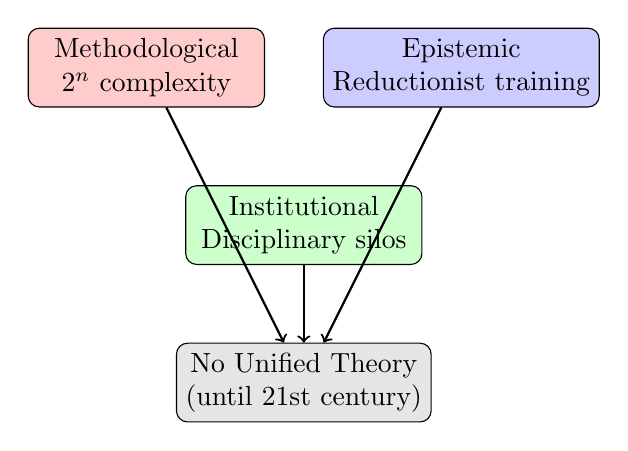
\begin{tikzpicture}[
    box/.style={rectangle, draw, rounded corners, minimum width=3cm, minimum height=1cm, align=center},
    arrow/.style={->, thick}
]
\node[box, fill=red!20] (method) at (0,2) {Methodological\\$2^n$ complexity};
\node[box, fill=blue!20] (epistemic) at (4,2) {Epistemic\\Reductionist training};
\node[box, fill=green!20] (institutional) at (2,0) {Institutional\\Disciplinary silos};
\node[box, fill=gray!20] (result) at (2,-2) {No Unified Theory\\(until 21st century)};

\draw[arrow] (method) -- (result);
\draw[arrow] (epistemic) -- (result);
\draw[arrow] (institutional) -- (result);
\end{tikzpicture}
\caption{Three Barriers to Unified Complementarity Theory}
\label{fig:three-barriers}
\end{figure}

% ============================================================================
% PART VIII: WHY NOW
% ============================================================================
\section{Phase VIII: Why the Time Is Now}
\label{sec:phase-viii}

\subsection{Conditions for Unification (2000--Present)}

\begin{tcolorbox}[colback=green!5!white,colframe=green!75!black,title=\textbf{Historical Diagnosis}]
For the first time in history, complementarity is:
\begin{itemize}[noitemsep]
    \item \textbf{Measurable:} Computational power enables estimation
    \item \textbf{Comparable:} Network theory provides common language
    \item \textbf{Modelable:} Machine learning handles interactions natively
    \item \textbf{Decision-relevant:} Complex interventions require $\gamma$ knowledge
\end{itemize}
\end{tcolorbox}

\subsubsection{Enabling Factor 1: Computational Power}

\textbf{Moore's Law consequences:}
\begin{itemize}[noitemsep]
    \item Factorial designs now computationally feasible
    \item Monte Carlo estimation of higher-order $\gamma$
    \item SHAP values calculable in real time
    \item Combinatorial optimization tractable
\end{itemize}

\textbf{Specific capability:} Estimate $\gamma$ from observational data via:
\begin{itemize}[noitemsep]
    \item Random forests with interaction detection
    \item Neural networks with interpretability
    \item Causal forests for heterogeneous effects
\end{itemize}

\subsubsection{Enabling Factor 2: Network Theory}

\textbf{The network revolution (1998--present):}
\begin{itemize}[noitemsep]
    \item Watts \& Strogatz: Small-world networks
    \item Barabási \& Albert: Scale-free networks
    \item Common mathematical language across domains
\end{itemize}

\textbf{Key insight:} Network edges \textit{are} complementarities.

\[
\text{Edge weight}_{ij} \approx \gamma_{ij}
\]

This provides a visual and mathematical common ground.

\subsubsection{Enabling Factor 3: Shapley Values and Game Theory}

\textbf{The SHAP revolution in ML:}
\begin{itemize}[noitemsep]
    \item Lundberg \& Lee (2017): Unified interpretability framework
    \item Shapley values decompose model predictions
    \item Interaction indices emerge naturally
\end{itemize}

\textbf{Mathematical foundation:}
\begin{align}
\phi_i &= \sum_{S \subseteq N \setminus \{i\}} \frac{|S|!(|N|-|S|-1)!}{|N|!} [v(S \cup \{i\}) - v(S)] \\
\phi_{ij} &= \text{Shapley interaction index}
\end{align}

This is exactly the EBF $\gamma$ in cooperative game form.

\subsubsection{Enabling Factor 4: Complex Data Availability}

\textbf{New data sources:}
\begin{itemize}[noitemsep]
    \item Genomics: Millions of gene combinations
    \item Neuroscience: Full brain connectivity maps
    \item Digital traces: Complete behavioral records
    \item A/B testing platforms: Factorial experiments at scale
\end{itemize}

\textbf{Consequence:} First time in history we can \textit{observe} complementarity structures at scale.

\subsubsection{Enabling Factor 5: Interdisciplinary Recognition}

\textbf{Signs of convergence:}
\begin{itemize}[noitemsep]
    \item Santa Fe Institute: Complexity science
    \item Network science journals accepting all domains
    \item ``Interaction'' as cross-disciplinary keyword
    \item Growing frustration with disciplinary fragmentation
\end{itemize}

\subsubsection{Summary: The Convergence Moment}

\begin{table}[h]
\centering
\caption{Why Now: Enabling Conditions}
\label{tab:why-now}
\renewcommand{\arraystretch}{1.3}
\begin{tabular}{@{}lccc@{}}
\toprule
\textbf{Factor} & \textbf{1990} & \textbf{2010} & \textbf{2025} \\
\midrule
Compute for $2^n$ & Limited & Improving & Sufficient \\
Network language & Absent & Emerging & Established \\
Shapley/SHAP & Unknown & Introduced & Standard \\
Big data & Rare & Growing & Ubiquitous \\
Cross-domain interest & Low & Moderate & High \\
\bottomrule
\end{tabular}
\end{table}

\begin{tcolorbox}[colback=yellow!5!white,colframe=yellow!75!black,title=\textbf{Historical Conclusion}]
The 2020s represent the \textbf{first moment in history} when a unified theory of complementarity is both:
\begin{enumerate}
    \item \textbf{Scientifically possible} (tools exist)
    \item \textbf{Practically necessary} (complex interventions demand it)
\end{enumerate}

This is the window the EBF $\gamma$-framework enters.
\end{tcolorbox}

% ============================================================================
% PART IX: POSITIONING THE EBF FRAMEWORK
% ============================================================================
\section{Phase IX: Historical Positioning of the $\gamma$-Framework}
\label{sec:phase-ix}

\subsection{EBF as Historical Culmination}

\begin{tcolorbox}[colback=blue!5!white,colframe=blue!75!black,title=\textbf{The $\gamma$-Framework's Historical Position}]
From a scientific-historical perspective, the EBF $\gamma$-framework represents:

\textbf{The first explicitly domain-general, formally unified, empirically operational theory of complementarity.}
\end{tcolorbox}

\subsubsection{What EBF Achieves That Predecessors Did Not}

\begin{table}[h]
\centering
\caption{EBF $\gamma$ vs. Historical Approaches}
\label{tab:ebf-vs-history}
\renewcommand{\arraystretch}{1.3}
\small
\begin{tabular}{@{}lccccc@{}}
\toprule
\textbf{Feature} & \textbf{Heraclitus} & \textbf{Bohr} & \textbf{Systems} & \textbf{Islands} & \textbf{EBF $\gamma$} \\
\midrule
Formal definition & $\times$ & $\times$ & $\times$ & \checkmark & \checkmark \\
Domain-general & \checkmark & $\times$ & \checkmark & $\times$ & \checkmark \\
Measurable & $\times$ & $\times$ & $\times$ & \checkmark & \checkmark \\
Unified notation & --- & --- & --- & $\times$ & \checkmark \\
Higher-order theory & --- & --- & --- & $\times$ & \checkmark \\
Intervention guidance & $\times$ & $\times$ & $\times$ & Partial & \checkmark \\
\bottomrule
\end{tabular}
\end{table}

\subsubsection{EBF's Unique Contributions}

\textbf{1. Universal Definition}
\[
\gamma_{ab} = f(\{a,b\}) - f(\{a\}) - f(\{b\}) + f(\emptyset)
\]

This single formula unifies:
\begin{itemize}[noitemsep]
    \item Economic complementarity (Topkis, Milgrom)
    \item Biological epistasis (Fisher, Phillips)
    \item Pharmacological synergy (Chou, Bliss)
    \item Statistical interactions (Fisher, ANOVA)
    \item ML feature interactions (SHAP)
\end{itemize}

\textbf{2. Hierarchical Extension}
\[
\gamma^L_{ab} = U^L(\{a,b\}) - U^L(\{a\}) - U^L(\{b\}) + U^L(\emptyset)
\]

Complementarity at multiple levels (individual, group, society)---not found in any predecessor.

\textbf{3. Domain Translation Maps}

Explicit mappings from universal $\gamma$ to:
\begin{itemize}[noitemsep]
    \item Economics: Cross-partial derivatives
    \item Psychology: Interaction effects
    \item Biology: Epistasis coefficients
    \item Pharmacology: Combination indices
\end{itemize}

See Appendix XII (DOMAIN-FOUND) for complete translation.

\textbf{4. Intervention Complementarity}

Application to behavioral interventions:
\[
\gamma_{\text{Nudge,Incentive}} = U(\text{N} + \text{I}) - U(\text{N}) - U(\text{I}) + U(\emptyset)
\]

Novel application not found in any historical treatment.

\subsubsection{Historical Lineage}

\begin{figure}[h]
\centering
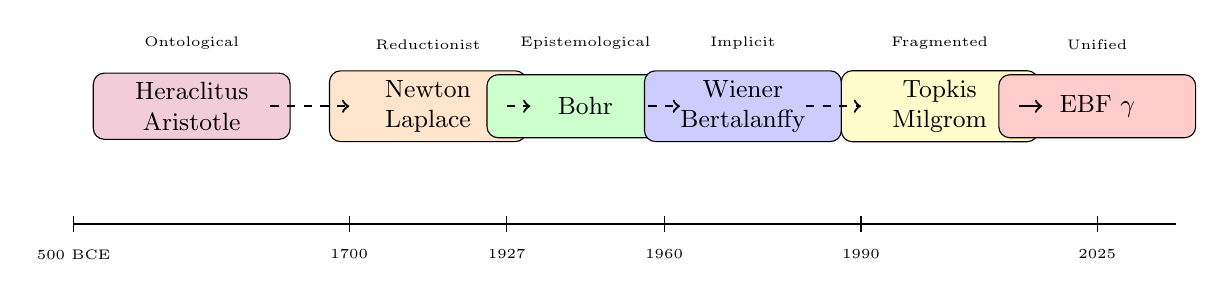
\begin{tikzpicture}[
    box/.style={rectangle, draw, rounded corners, minimum width=2.5cm, minimum height=0.8cm, align=center, font=\small},
    arrow/.style={->, thick}
]
% Timeline
\draw[thick] (0,0) -- (14,0);
\foreach \x/\label in {0/500 BCE, 3.5/1700, 5.5/1927, 7.5/1960, 10/1990, 13/2025} {
    \draw (\x,0.1) -- (\x,-0.1);
    \node[below, font=\tiny] at (\x,-0.2) {\label};
}

% Boxes
\node[box, fill=purple!20] at (1.5,1.5) {Heraclitus\\Aristotle};
\node[box, fill=orange!20] at (4.5,1.5) {Newton\\Laplace};
\node[box, fill=green!20] at (6.5,1.5) {Bohr};
\node[box, fill=blue!20] at (8.5,1.5) {Wiener\\Bertalanffy};
\node[box, fill=yellow!20] at (11,1.5) {Topkis\\Milgrom};
\node[box, fill=red!20] at (13,1.5) {EBF $\gamma$};

% Arrows
\draw[arrow, dashed] (2.5,1.5) -- (3.5,1.5);
\draw[arrow, dashed] (5.5,1.5) -- (5.8,1.5);
\draw[arrow, dashed] (7.3,1.5) -- (7.7,1.5);
\draw[arrow, dashed] (9.3,1.5) -- (10,1.5);
\draw[arrow] (12,1.5) -- (12.3,1.5);

% Labels
\node[above, font=\tiny] at (1.5,2.1) {Ontological};
\node[above, font=\tiny] at (4.5,2.1) {Reductionist};
\node[above, font=\tiny] at (6.5,2.1) {Epistemological};
\node[above, font=\tiny] at (8.5,2.1) {Implicit};
\node[above, font=\tiny] at (11,2.1) {Fragmented};
\node[above, font=\tiny] at (13,2.1) {Unified};
\end{tikzpicture}
\caption{Historical Trajectory of Complementarity Science}
\label{fig:historical-trajectory}
\end{figure}

\subsubsection{The $\gamma$-Framework as Paradigm Shift}

In Kuhnian terms, the EBF $\gamma$-framework represents:

\begin{itemize}
    \item \textbf{Not} a revolution within a discipline (that was Topkis, Milgrom)
    \item \textbf{But} a meta-paradigm unifying previously separate sciences
\end{itemize}

\begin{quote}
``Complementarity was always intuitively plausible, long philosophically accepted, seldom formalized---and only now scientifically mature.''
\end{quote}

% ============================================================================
% SUMMARY
% ============================================================================
\section{Summary: The 2,500-Year Journey}
\label{sec:summary}

\begin{tcolorbox}[colback=gray!5!white,colframe=gray!75!black,title=\textbf{Historical Summary}]

\renewcommand{\arraystretch}{1.4}
\begin{tabular}{@{}clll@{}}
\toprule
\textbf{Phase} & \textbf{Period} & \textbf{Achievement} & \textbf{Limitation} \\
\midrule
I & Antiquity--1600 & Ontological intuition & Not scientific \\
II & 1600--1920 & (Reductionist detour) & Complementarity suppressed \\
III & 1920--1940 & Epistemological articulation & Not generalizable \\
IV & 1940--1970 & Systemic recognition & Not formalized \\
V & 1970--2000 & Disciplinary formalization & Not unified \\
VI & 2000--2020 & Computational enablement & Still fragmented \\
VII & 2020--present & \textbf{Unification possible} & \textbf{EBF $\gamma$} \\
\bottomrule
\end{tabular}

\vspace{1em}
\textbf{The EBF Framework's Historical Achievement:}

Converting 2,500 years of intuition into operational science.
\end{tcolorbox}

% ============================================================================
% GLOSSARY
% ============================================================================
\section{Glossary}
\label{sec:glossary}

Key terms in this appendix (see also Appendix G for complete glossary):

\begin{description}[style=nextline]
    \item[Complementarity] Non-additive interaction: $\gamma = f(A \cup B) - f(A) - f(B) + f(\emptyset)$
    \item[Reductionism] Methodological assumption that wholes equal sum of parts
    \item[Supermodularity] Global positive complementarity on a lattice (Topkis)
    \item[Epistasis] Genetic complementarity between mutations
    \item[Bohrian Complementarity] Mutual exclusivity of quantum descriptions
    \item[Systems Theory] Study of emergent properties from component interactions
    \item[Formal Island] Disciplinary formalization without cross-domain integration
    \item[Shapley Value] Fair allocation based on marginal contributions
    \item[SHAP] SHapley Additive exPlanations (ML interpretability)
\end{description}

% ============================================================================
% REFERENCES
% ============================================================================
\section{Scientific References}
\label{sec:references}

This section documents the scientific history with primary sources organized by historical phase.

\subsection{Phase I: Pre-Scientific Sources (8 works)}

\begin{enumerate}
    \item Heraclitus (c. 500 BCE). Fragments. In: Kirk, G.S., Raven, J.E., \& Schofield, M. (1983). \textit{The Presocratic Philosophers} (2nd ed.). Cambridge University Press.

    \item Aristotle (c. 350 BCE). \textit{Metaphysics}. Translated by W.D. Ross (1924). Oxford: Clarendon Press.

    \item Aristotle (c. 350 BCE). \textit{Physics}. Translated by R. Waterfield (1996). Oxford University Press.

    \item Laozi (c. 400 BCE). \textit{Tao Te Ching}. Various translations.

    \item Nicholas of Cusa (1440). \textit{De docta ignorantia}. Translated as \textit{On Learned Ignorance} by J. Hopkins (1981). Minneapolis: Banning Press.

    \item Aquinas, T. (1265--1274). \textit{Summa Theologica}. Various editions.

    \item Granet, M. (1934). \textit{La pensée chinoise}. Paris: Albin Michel. [On Yin-Yang]

    \item Lloyd, G.E.R. (1966). \textit{Polarity and Analogy}. Cambridge University Press.
\end{enumerate}

\subsection{Phase II: Classical Science (6 works)}

\begin{enumerate}
    \setcounter{enumi}{8}
    \item Newton, I. (1687). \textit{Philosophiae Naturalis Principia Mathematica}. London.

    \item Laplace, P.-S. (1814). \textit{Essai philosophique sur les probabilités}. Paris.

    \item Cournot, A.A. (1838). \textit{Recherches sur les principes mathématiques de la théorie des richesses}. Paris. [First mathematical complementarity]

    \item Cuvier, G. (1812). \textit{Recherches sur les ossemens fossiles}. Paris. [Correlation of parts]

    \item Mill, J.S. (1843). \textit{A System of Logic}. London: Longmans. [Composition of causes]

    \item Duhem, P. (1906). \textit{La théorie physique: son objet et sa structure}. Paris. [Holism in physics]
\end{enumerate}

\subsection{Phase III: Quantum Complementarity (8 works)}

\begin{enumerate}
    \setcounter{enumi}{14}
    \item Bohr, N. (1928). The quantum postulate and the recent development of atomic theory. \textit{Nature}, 121, 580--590.

    \item Bohr, N. (1934). \textit{Atomic Theory and the Description of Nature}. Cambridge University Press.

    \item Bohr, N. (1958). \textit{Atomic Physics and Human Knowledge}. New York: Wiley.

    \item Heisenberg, W. (1927). Über den anschaulichen Inhalt der quantentheoretischen Kinematik und Mechanik. \textit{Zeitschrift für Physik}, 43, 172--198.

    \item Pauli, W., \& Jung, C.G. (1952). \textit{The Interpretation of Nature and the Psyche}. New York: Pantheon.

    \item Jammer, M. (1974). \textit{The Philosophy of Quantum Mechanics}. New York: Wiley.

    \item Folse, H.J. (1985). \textit{The Philosophy of Niels Bohr}. Amsterdam: North-Holland.

    \item Murdoch, D. (1987). \textit{Niels Bohr's Philosophy of Physics}. Cambridge University Press.
\end{enumerate}

\subsection{Phase IV: Systems Theory (8 works)}

\begin{enumerate}
    \setcounter{enumi}{22}
    \item Wiener, N. (1948). \textit{Cybernetics: Control and Communication in the Animal and the Machine}. MIT Press.

    \item Bertalanffy, L. von (1968). \textit{General System Theory}. New York: Braziller.

    \item Ashby, W.R. (1956). \textit{An Introduction to Cybernetics}. London: Chapman \& Hall.

    \item Ashby, W.R. (1952). \textit{Design for a Brain}. London: Chapman \& Hall.

    \item Bateson, G. (1972). \textit{Steps to an Ecology of Mind}. San Francisco: Chandler.

    \item Luhmann, N. (1984). \textit{Soziale Systeme}. Frankfurt: Suhrkamp. [English: 1995, Stanford]

    \item Maturana, H., \& Varela, F. (1980). \textit{Autopoiesis and Cognition}. Dordrecht: Reidel.

    \item Prigogine, I., \& Stengers, I. (1984). \textit{Order Out of Chaos}. New York: Bantam.
\end{enumerate}

\subsection{Phase V: Formal Islands---Economics (10 works)}

\begin{enumerate}
    \setcounter{enumi}{30}
    \item Leontief, W. (1941). \textit{The Structure of the American Economy, 1919--1939}. Oxford University Press.

    \item Topkis, D.M. (1978). Minimizing a submodular function on a lattice. \textit{Operations Research}, 26(2), 305--321.

    \item Topkis, D.M. (1998). \textit{Supermodularity and Complementarity}. Princeton University Press.

    \item Milgrom, P., \& Roberts, J. (1990). The economics of modern manufacturing. \textit{American Economic Review}, 80(3), 511--528.

    \item Milgrom, P., \& Roberts, J. (1995). Complementarities and fit: Strategy, structure, and organizational change in manufacturing. \textit{Journal of Accounting and Economics}, 19(2--3), 179--208.

    \item Milgrom, P., \& Shannon, C. (1994). Monotone comparative statics. \textit{Econometrica}, 62(1), 157--180.

    \item Vives, X. (1990). Nash equilibrium with strategic complementarities. \textit{Journal of Mathematical Economics}, 19(3), 305--321.

    \item Athey, S. (2002). Monotone comparative statics under uncertainty. \textit{Quarterly Journal of Economics}, 117(1), 187--223.

    \item Amir, R. (2005). Supermodularity and complementarity in economics. \textit{Journal of Economic Literature}, 43(3), 783--804.

    \item Brynjolfsson, E., \& Milgrom, P. (2013). Complementarity in organizations. In R. Gibbons \& J. Roberts (Eds.), \textit{Handbook of Organizational Economics}. Princeton University Press.
\end{enumerate}

\subsection{Phase V: Formal Islands---Biology (8 works)}

\begin{enumerate}
    \setcounter{enumi}{40}
    \item Fisher, R.A. (1918). The correlation between relatives on the supposition of Mendelian inheritance. \textit{Transactions of the Royal Society of Edinburgh}, 52, 399--433.

    \item Hill, A.V. (1910). The possible effects of the aggregation of the molecules of haemoglobin on its dissociation curves. \textit{Journal of Physiology}, 40, iv--vii.

    \item Monod, J., Wyman, J., \& Changeux, J.-P. (1965). On the nature of allosteric transitions. \textit{Journal of Molecular Biology}, 12, 88--118.

    \item Phillips, P.C. (2008). Epistasis---the essential role of gene interactions in the structure and evolution of genetic systems. \textit{Nature Reviews Genetics}, 9(11), 855--867.

    \item Weinreich, D.M., et al. (2013). Should evolutionary geneticists worry about higher-order epistasis? \textit{Current Opinion in Genetics \& Development}, 23(6), 700--707.

    \item Tilman, D., et al. (1996). Productivity and sustainability influenced by biodiversity in grassland ecosystems. \textit{Nature}, 379, 718--720.

    \item Loreau, M., \& Hector, A. (2001). Partitioning selection and complementarity in biodiversity experiments. \textit{Nature}, 412, 72--76.

    \item Beerenwinkel, N., Pachter, L., \& Sturmfels, B. (2007). Epistasis and shapes of fitness landscapes. \textit{Statistica Sinica}, 17(4), 1317--1342.
\end{enumerate}

\subsection{Phase V: Formal Islands---Pharmacology (4 works)}

\begin{enumerate}
    \setcounter{enumi}{48}
    \item Bliss, C.I. (1939). The toxicity of poisons applied jointly. \textit{Annals of Applied Biology}, 26, 585--615.

    \item Loewe, S. (1953). The problem of synergism and antagonism of combined drugs. \textit{Arzneimittel-Forschung}, 3, 285--290.

    \item Chou, T.-C., \& Talalay, P. (1984). Quantitative analysis of dose-effect relationships. \textit{Advances in Enzyme Regulation}, 22, 27--55.

    \item Chou, T.-C. (2006). Theoretical basis, experimental design, and computerized simulation of synergism and antagonism. \textit{Pharmacological Reviews}, 58(3), 621--681.
\end{enumerate}

\subsection{Phase VI: Enabling Technologies (10 works)}

\begin{enumerate}
    \setcounter{enumi}{52}
    \item Watts, D.J., \& Strogatz, S.H. (1998). Collective dynamics of `small-world' networks. \textit{Nature}, 393, 440--442.

    \item Barabási, A.-L., \& Albert, R. (1999). Emergence of scaling in random networks. \textit{Science}, 286, 509--512.

    \item Shapley, L.S. (1953). A value for $n$-person games. In H.W. Kuhn \& A.W. Tucker (Eds.), \textit{Contributions to the Theory of Games II}. Princeton University Press.

    \item Lundberg, S.M., \& Lee, S.-I. (2017). A unified approach to interpreting model predictions. \textit{NeurIPS}, 4765--4774.

    \item Wager, S., \& Athey, S. (2018). Estimation and inference of heterogeneous treatment effects using random forests. \textit{JASA}, 113(523), 1228--1242.

    \item Nemhauser, G.L., Wolsey, L.A., \& Fisher, M.L. (1978). An analysis of approximations for maximizing submodular set functions. \textit{Mathematical Programming}, 14(1), 265--294.

    \item Krause, A., \& Golovin, D. (2014). Submodular function maximization. In \textit{Tractability} (pp. 71--104). Cambridge University Press.

    \item Grabisch, M. (2016). \textit{Set Functions, Games and Capacities in Decision Making}. Springer.

    \item Athey, S., \& Imbens, G.W. (2019). Machine learning methods that economists should know about. \textit{Annual Review of Economics}, 11, 685--725.

    \item Lou, Y., et al. (2013). Accurate intelligible models with pairwise interactions. \textit{KDD}, 623--631.
\end{enumerate}

\subsection{Historiography and Philosophy of Science (6 works)}

\begin{enumerate}
    \setcounter{enumi}{62}
    \item Kuhn, T.S. (1962). \textit{The Structure of Scientific Revolutions}. Chicago: University of Chicago Press.

    \item Lakatos, I. (1978). \textit{The Methodology of Scientific Research Programmes}. Cambridge University Press.

    \item Galison, P. (1997). \textit{Image and Logic}. Chicago: University of Chicago Press. [Trading zones between sciences]

    \item Hacking, I. (1983). \textit{Representing and Intervening}. Cambridge University Press.

    \item Dear, P. (2006). \textit{The Intelligibility of Nature}. Chicago: University of Chicago Press.

    \item Daston, L., \& Galison, P. (2007). \textit{Objectivity}. New York: Zone Books.
\end{enumerate}

\subsection{Reference Summary}

\begin{table}[h]
\centering
\caption{Distribution of References by Phase}
\label{tab:ref-summary}
\renewcommand{\arraystretch}{1.2}
\begin{tabular}{@{}lr@{}}
\toprule
\textbf{Historical Phase} & \textbf{Works} \\
\midrule
Phase I: Pre-Scientific & 8 \\
Phase II: Classical Science & 6 \\
Phase III: Quantum/Bohr & 8 \\
Phase IV: Systems Theory & 8 \\
Phase V: Economics & 10 \\
Phase V: Biology & 8 \\
Phase V: Pharmacology & 4 \\
Phase VI: Enabling Technologies & 10 \\
Historiography & 6 \\
\midrule
\textbf{Total} & \textbf{68} \\
\bottomrule
\end{tabular}
\end{table}

% ============================================================================
% CONCLUDING STATEMENT
% ============================================================================
\begin{tcolorbox}[colback=blue!5!white,colframe=blue!75!black,title=\textbf{Concluding Historical Statement}]
\begin{center}
\large
\textit{``Complementarity was always intuitively plausible,\\
long philosophically accepted,\\
seldom formalized---\\
and only now scientifically mature.''}
\end{center}

\vspace{0.5em}
The EBF $\gamma$-framework represents the culmination of a 2,500-year intellectual trajectory---from Heraclitus's unity of opposites to a formal, domain-general, empirically operational theory of interaction.
\end{tcolorbox}

\end{chapter}
